\chapter{StencilFlow Architecture Model}
One the one hand, field programmable gate arrays give us much higher flexibility compared to traditional computed devices such as central progressing units or graphics processing units. On the other hand, a good strategy and knowledge about the underlying hardware is required in order to make use of this additional degrees of freedom.\\
This section is dedicated to outline theoretical aspects of the overall strategy we are proposing. This includes the transformation from the abstracted high-level theoretical input to the mapping onto the actual hardware resources. 



\section{Application Specific Dataflow for Weather Codes}
Kernel computations on structured grids usually impose high stress on data movement since the amount of actual computations is rather low. Therefore we seek to transform the problem to a single, deep pipeline. This allows us to directly forward the intermediate result of a compute unit to the next   unit, instead of transferring it back to slow memory (or some intermediate cache) and later fetch it again. This optimization technique is widely used in hardware designs and not only increases the efficient usage of the resources, but can also save energy by not involving the lower memory hierarchy.\\
As we will see later on, larger designs with more complex dependencies might impose constraints such that we are not always able to directly forward the result to the next processing unit. Therefore we have to statically analyze where and in which size we have to allocate buffers for temporary storing the intermediate results. Since fast memory is limited, we have to find a good strategy to decide whether or not to use fast memory for a buffer allocation or sacrifice memory bandwidth and swap the buffer out to slow memory.


\subsection{Example Walk-through}
To better understand what this means in practice, we will go through the transformation of a simple two kernel example stencil program and its transformation to a fully pipelined design. \\
The stencil program illustrated in figure \ref{fig:approach-stencil-program} consists of three input data arrays (inA, inB, inC), a first kernel kernelA reading from inA and inB a second kernel kernelB reading from inC and kernelA. The final result is the output of kernelB. \\
\begin{lstlisting}[showstringspaces=false, frame=single, language=Python, label={lst:example-stencil-program}]     
inputs: inA, inB, inC
outputs: kernelB
kernels:
kernelA[i,j,k] = (inA[i,j,k]+inA[i,j,k+1])*inB[i,j,k]
kernelB[i,j,k] = (1.0-inC[i,j,k])*kernelA[i,j,k]
\end{lstlisting}
\begin{figure}[h]
	\centering
	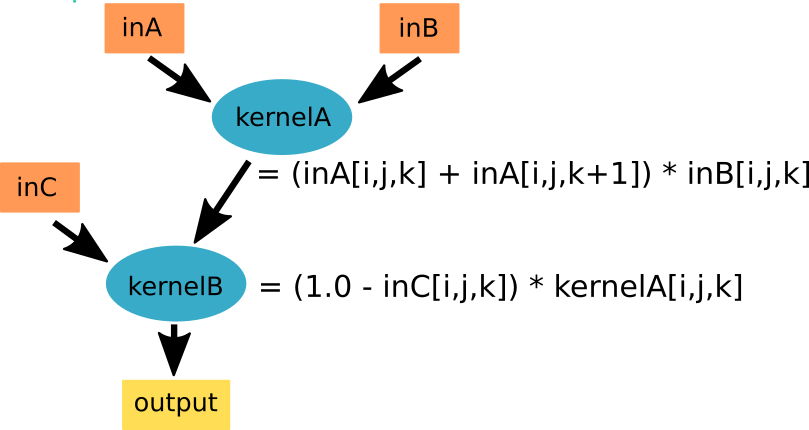
\includegraphics[height=12em]{drawings/approach-stencil-program.png}
	\caption{Example stencil program in high-level data flow representation.}
	\label{fig:approach-stencil-program}
\end{figure}

To avoid storing results of kernelA back to memory, we can directly forward the result to kernelB as illustrated in listing.
\begin{lstlisting}[showstringspaces=false, frame=single, language=Python, label={lst:example-stencil-program-substituted}]     
inputs: inA, inB, inC
outputs: kernelB
kernels:
kernelB[i,j,k] = (1.0 - inC[i,j,k])*(inA[i,j,k] +
                 inA[i,j,k+1])*inB[i,j,k]
\end{lstlisting}
This expression can then be laid down in a pipeline manner by following the mathematical precedence rule of the operation shown in figure \ref{fig:approach-stencil-program-pipeline}.
\begin{figure}[h]
	\centering
	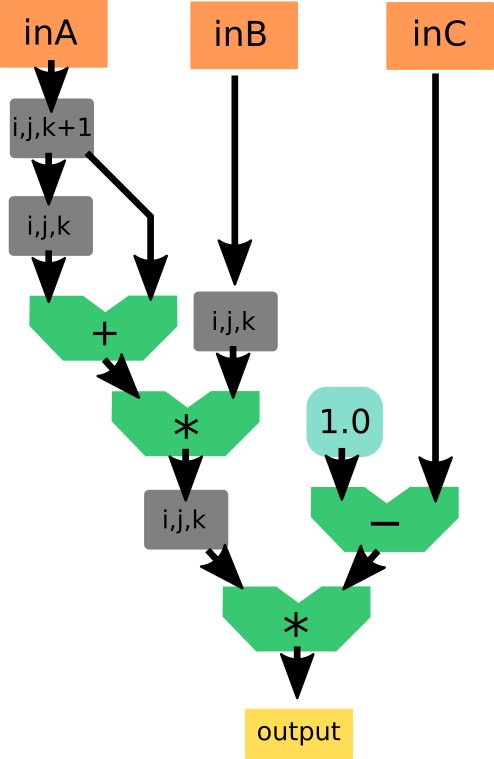
\includegraphics[height=16em]{drawings/approach-stencil-program-pipeline.png}
	\caption{Example stencil program visualized as a pipeline.}
	\label{fig:approach-stencil-program-pipeline}
\end{figure}
Since we are reading two fields from inA with an offset of one, we have to add a stage where we buffer the element at [i,j,k] first in order to be able to read both data elements simultaneously. \\
When we look from a higher level at the pipeline again, illustrated in figure \ref{fig:approach-stencil-program-pipeline-annotated}, we can see the major components:
\begin{itemize}
	\item Inputs: the input data arrays: inA, inB, inC
	\item Kernels: the two compute kernels: kernelA, kernelB
	\item Output: the output data store with the compute result: output
	\item a channel that transfers data from the first to the second kernel
\end{itemize}

\begin{figure}[h]
	\centering
	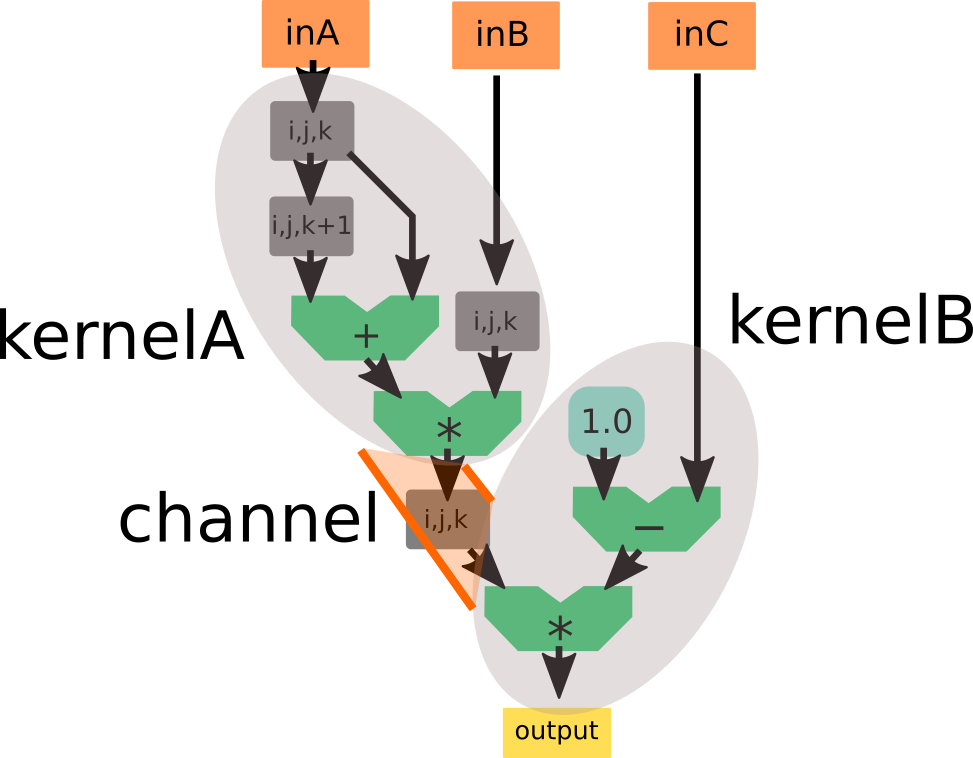
\includegraphics[height=16em]{drawings/approach-stencil-program-pipeline-annotated.png}
	\caption{Example stencil program with additional annotation about the structure of kernels and channels connecting the kernels.}
	\label{fig:approach-stencil-program-pipeline-annotated}
\end{figure}
As we will see later on, this structure builds the foundation for further analysis.


\subsection{Reason}
There are several reasons why we think that deep pipelining is the right choice. First, todays FPGAs are very well suited and optimized to generate highly efficient and higher-frequency designs compared to earlier re-programmable hardware logic designs \cite{label55,label56}. In addition, the incorporated hard compute units have a raw peak performances of 10 TFLOP/s of 32-bit single precision floating point compute performance.\\  
Furthermore, pipelining can save us a lot of data movements since we can directly forward the result of the previous computation to the next compute unit. This can significantly increase performance in case of memory bottlenecks and the idling time associated with it.


\paragraph{}
We conclude that the actual problem is about optimal allocation of the different resources for maximizing the overall throughput. This brings us to the question of, given an stencil program, which and how much resources are required to implement it efficiently in hardware. The next section is dedicated to this input problem analysis. 





\section{Analysis}
This section is dedicated to find and formalize the key metrics for transforming an input problem to a fully pipelined design. We reason about how different patterns of the input program require certain resources such as buffer space and generalize this in order to make these analysis steps fully automatic by StencilFlow.\\
As we have seen in the previous section, it naturally makes sense to split the stencil program into inputs, kernels and outputs. We will therefore first look at the individual kernels and later on use the information and insights gained from this to reason about the whole stencil program.


\subsection{Kernel}
The base of a kernel consists of a kernel string or mathematical expression, the actual stencil. We are dealing with shift-invariant stencils that can read from a neighborhood of the center element [i,j,k] to produce the result for the data element at [i,j,k]. This stencil pattern is then applied for the elements in the grid.\\
The key metrics we are interested in is the latency of a single computation given the latency of each individual operation and the amount of buffer space required such that we do not have to re-fetch the same data element for the stencil twice. We will refer to this as the internal buffer and derive the formula for its size in this section. \\


\paragraph{Stencil}
Shift-invariant stencils are operators that perform element-wise computation of a function F over a fixed neighborhood S. Therefore they can be element-wise applied to each location of the data grid as illustrated in figures \ref{fig:model-stencil-general} and \ref{fig:model-stencil2}. 

\begin{minted}{python}
for i=1..N
  for j=1..M
    out(i,j) = F(S(i,j))
\end{minted}
\begin{align}
\text{S}(i,j) = \text{in}(u,v)
\text{, (u,v)} \in \{(i,j), (i,j-1), (i,j+1), (i-1,j), (i+1,j)\}
\end{align}
\begin{align}
\text{F: } \mathbb{R}^{|S|} \rightarrow \mathbb{R}
\end{align}



\begin{figure}[h]
	\begin{minipage}{.5\columnwidth}
		\centering
		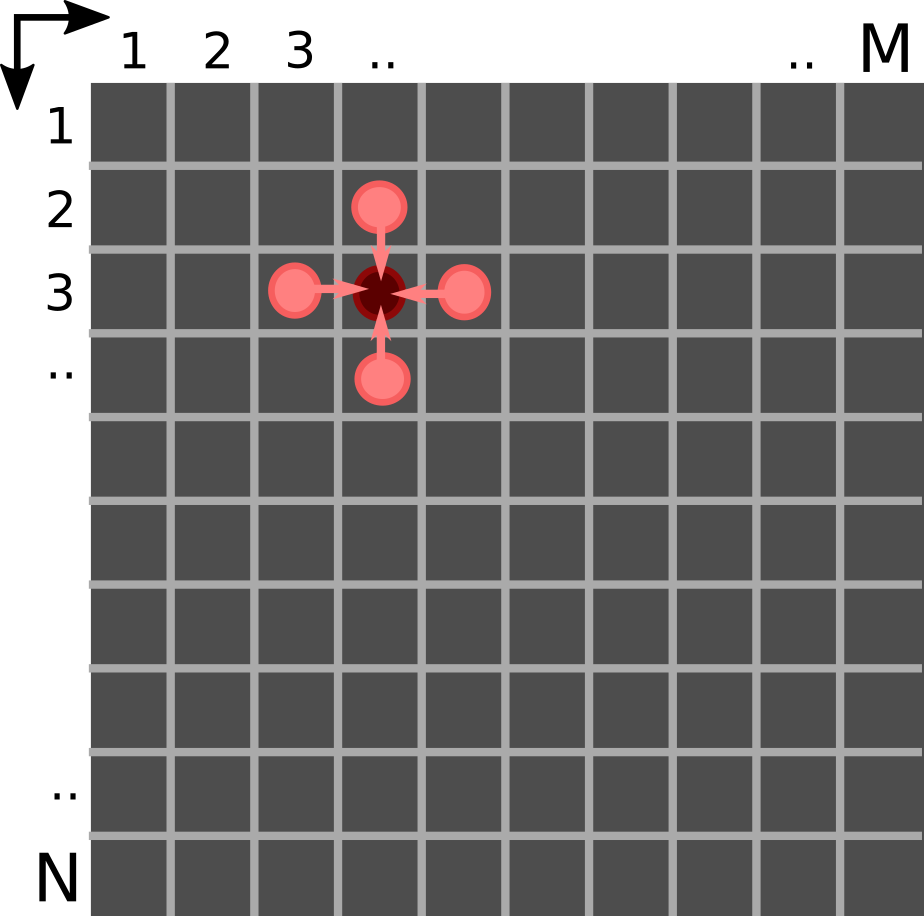
\includegraphics[height=16em]{drawings/model-stencil-general.png}
		\caption{A two dimensional stencil laid out on a two dimensional grid.}
		\label{fig:model-stencil-general}
		\vspace{1em}
	\end{minipage}
	\begin{minipage}{.5\columnwidth}
		\centering
		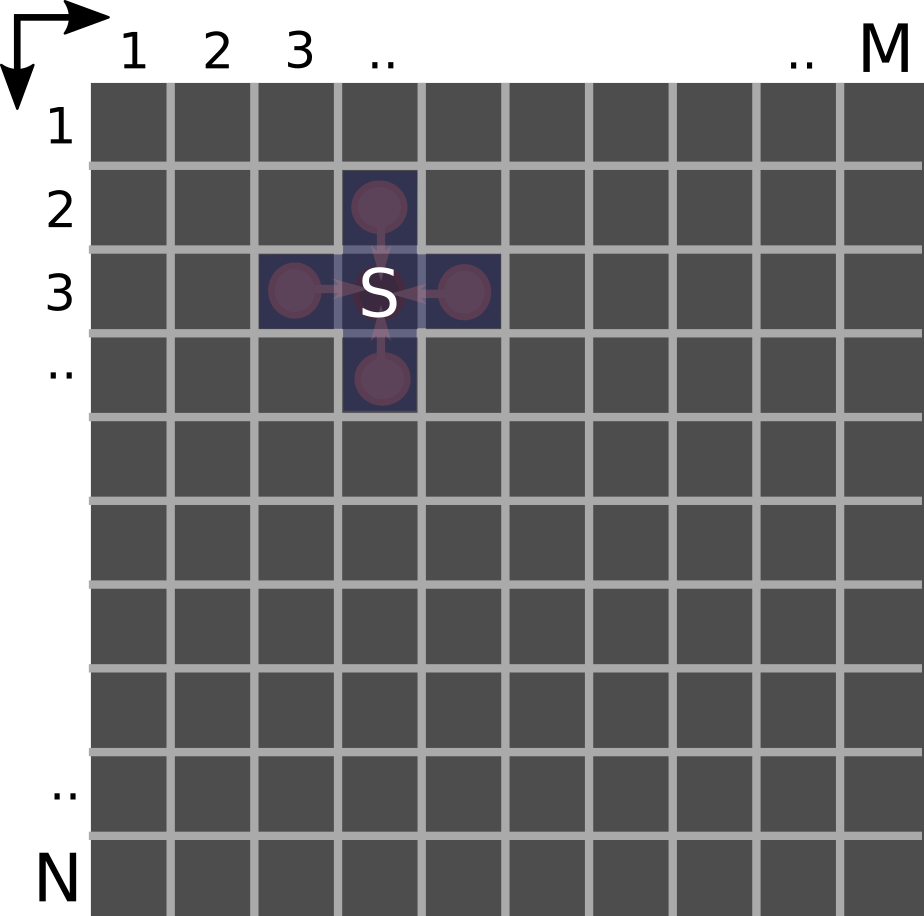
\includegraphics[height=16em]{drawings/model-stencil-neighbourhood-array.png}
		\caption{A two dimensional stencil laid out on a two dimensional grid with emphasized neighborhood S.}
		\label{fig:model-stencil2}
	\end{minipage}
\end{figure}



\subparagraph{Boundary Conditions}
At the boundary of the grid shown in figure \ref{fig:model-boundary-condition1}, some accesses of the neighborhood might be out-of-bound. For this special case, there are different strategies that can be applied to pad the grid shown in figure \ref{fig:model-boundary-condition2}. \\
The most commonly used ones are constant, copy and interpolation boundary conditions. The constant boundary condition assigns a pre-defined constant value to each out-of-bound data access. The copy boundary condition copies the value of the last valid access field and the interpolation boundary condition interpolates the value from some neighborhood around the boundary (e.g. polynomial of degree one or two).
\begin{figure}[H]
	\begin{minipage}{.5\columnwidth}
		\centering
		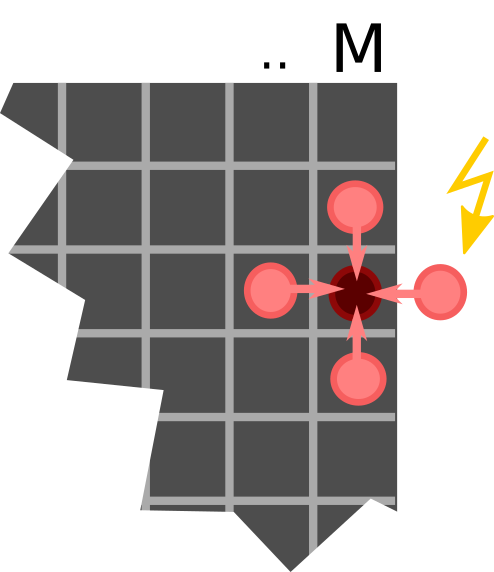
\includegraphics[height=12em]{drawings/model-boundary-condition1.png}
		\caption{Example case of a field access outside of the data array.}
		\label{fig:model-boundary-condition1}
		\vspace{1em}
	\end{minipage}
	\begin{minipage}{.5\columnwidth}
		\centering
		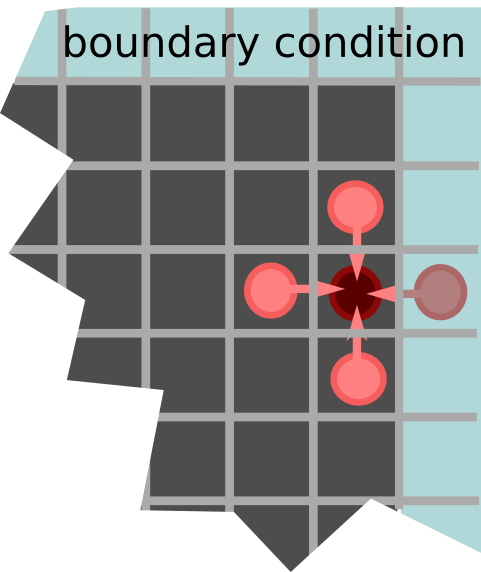
\includegraphics[height=12em]{drawings/model-boundary-condition2.png}
		\caption{Example case of a field access outside of the data array with emphasized boundary condition.}
		\label{fig:model-boundary-condition2}
	\end{minipage}
\end{figure}



\paragraph{Compute Graph}
We represent these computations as an abstract syntax tree graph consisting of input nodes, operation nodes and output nodes. \\
The input nodes feed data into the compute graph and are either constant numerals, variables or array field accesses. The operation nodes represent the actual compute units. They can be binary operations such as addition and multiplication, but also unary operations (e.g. negation), function calls (e.g. sin/cos) or the ternary operator. At the end (or root of the tree) of the compute graph is always an output node that carries the actual computation result as shown in figure \ref{fig:implementation-compute-graph}. 
\begin{minted}{c++}
res = (1.0 > c*d) ? (a-b):(c*d) 
\end{minted}
\begin{figure}[H]
	\centering
	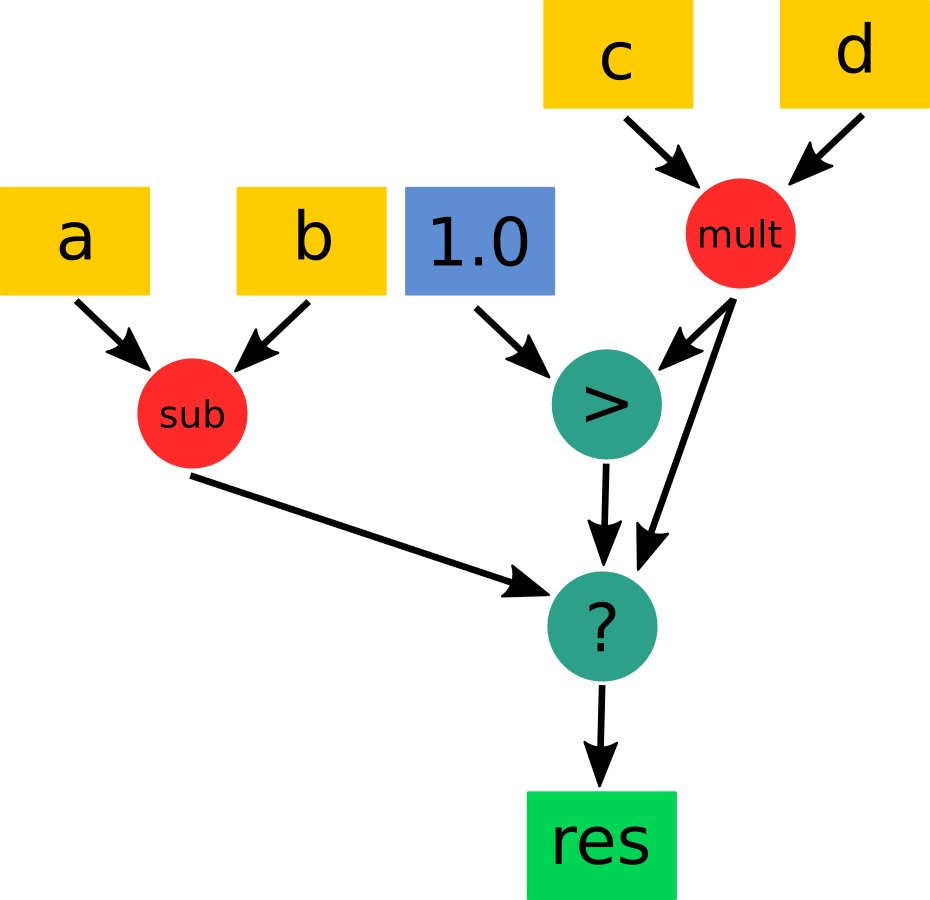
\includegraphics[height=16em]{drawings/implementation-compute-graph.png}
	\caption{Example Compute Graph.}
	\label{fig:implementation-compute-graph}
\end{figure}


\paragraph{Latency}
In order to compute the global stencil program latency, we are interested in the critical path latency of each individual stencil. Using the graph representation of the AST and a static mapping of each operation to the number of cycles it takes to perform a single operation, we can simply walk up the tree from the result and sum up the latency of each computation node till an input node is being reached. The highest latency value at some input corresponds to the overall critical path latency of the stencil.


\paragraph{Internal Buffer} \label{para:internal-buffer}
We refer to the internal buffer as the buffer space required such that each input data element has to be fetched or read only once. In other words, we want to store all data elements once they have been used for the first time by this specific stencil till they retire (not being required any longer) as shown in figure \ref{fig:model-internal-buffer}. \\
To get a good understanding, we derive the formula of this calculation by looking at some examples. Without loss of generality, we assume that we have a single three dimensional input data grid that we are looping over (figure \ref{fig:buffer-array}) using our stencil where the center element of the stencil is the field we are producing the result for. The derived formula can be extended to multiple different input arrays by splitting the field accesses for each input array and solve the problem for each of them. Furthermore, we iterate over the array in the following dimensional order:
\begin{minted}{python}
for i=1..Z
  for j=1..Y
    for k=1..X
\end{minted}


\begin{figure}[h]
	\begin{minipage}{.5\columnwidth}
	\centering
	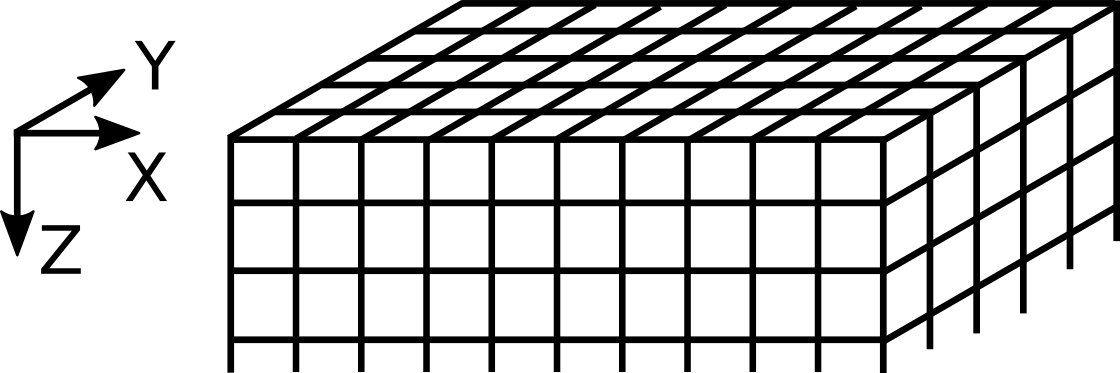
\includegraphics[height=5.5em]{drawings/buffer-array.png}
	\caption{Data array.}
	\label{fig:buffer-array}
	\vspace{-10.5em}
	\end{minipage}
	\begin{minipage}{.5\columnwidth}
	\centering
	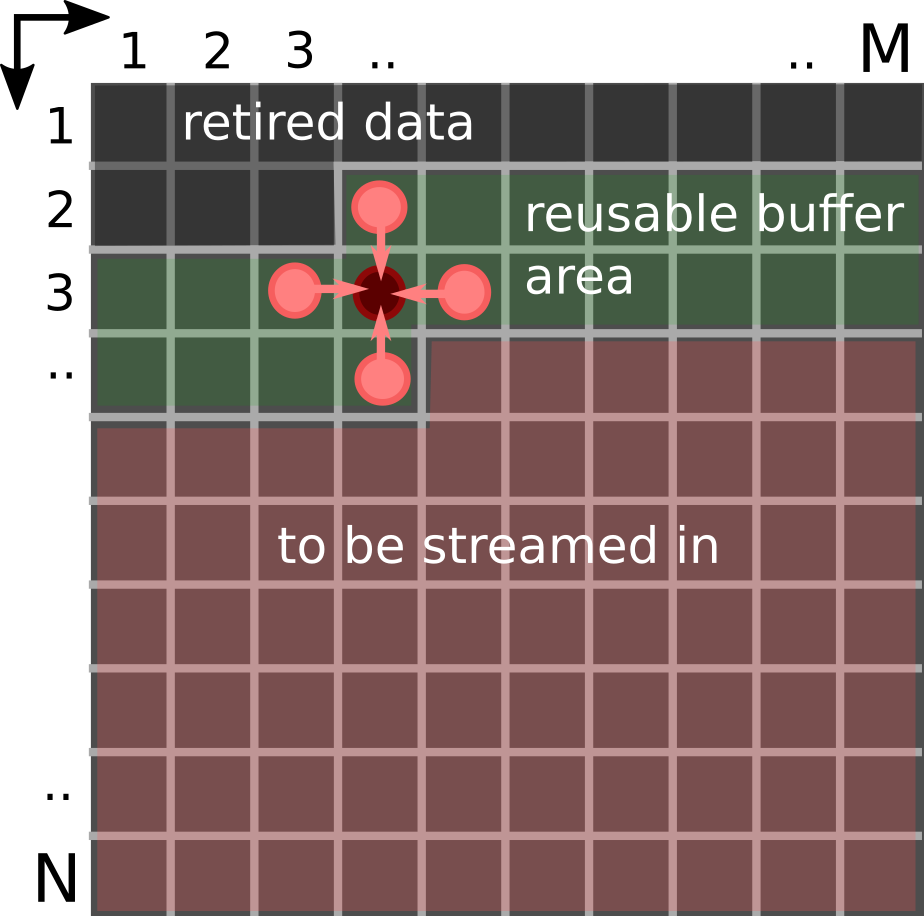
\includegraphics[height=16em]{drawings/model-internal-buffer.png}
	\caption{Internal Buffer of a Stencil.}
	\label{fig:model-internal-buffer}
	\end{minipage}
\end{figure}


\subparagraph{Example 1: Single Element}
Our first example is a kernel that simply multiplies the only input element by a factor of 7.0. Furthermore, the only field access is at the same location on the grid as we write the output to (at [i,j,k]). 
\begin{align}
\text{out}(i, j, k) = 7.0 \cdot \text{in}(i, j, k)
\end{align}
This leads to a stencil consisting only of a single element (namely the center element itself) as illustrated in figure \ref{fig:buffer-ex1-no-buffer}. \\
Figure \ref{fig:buffer-ex1-buffer} shows the internal buffer of such a stencil operator, which is one data element wide. As soon as the data element has been read, it will not be used anymore and it can therefore be discarded. \\
\begin{figure}[h]
	\begin{minipage}{.5\columnwidth}
		\centering
		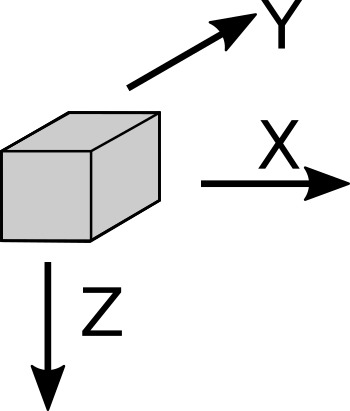
\includegraphics[height=12em]{drawings/buffer-ex1-no-buffer.png}
		\caption{Example 1: Stencil Operator.}
		\label{fig:buffer-ex1-no-buffer}
	\end{minipage}
	\begin{minipage}{.5\columnwidth}
		\centering
		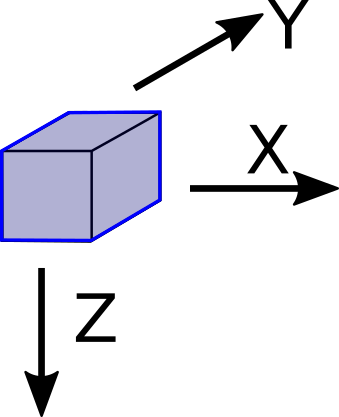
\includegraphics[height=12em]{drawings/buffer-ex1-buffer.png}
		\caption{Example 1: Internal Buffer laid over the Stencil.}
		\label{fig:buffer-ex1-buffer}
	\end{minipage}
\end{figure}

This number can also be derived by computing the difference between the highest and the lowest access index and adding one.
\begin{align}
\text{max index} - \text{min index} + 1 = [i, j, k] - [i, j, k] + 1 = [0, 0, 0] + 1
\end{align}
We will check with more complex examples if the formula also holds for them.\\


\subparagraph{Example 2: 1D Stencil}
Our second example consists of a stencil that sums over the center element and its predecessor and successor element in X direction. 
\begin{align}
\text{out}(i, j, k) = \text{in}(i, j, k-1) + \text{in}(i, j, k) + \text{in}(i, j, k+1)
\end{align}
Therefore, the stencil consists of three cubes (figure \ref{fig:buffer-ex2-no-buffer}) laid out next to each other in the direction of the X axis.\\
The internal buffer size of such a stencil operator is three data element wide. This can be verified by hand since we are in the innermost loop and the stencil therefore moves forward each iteration by one element in X direction. Therefore, the element read by the field access [i,j,k+1] can be discarded after the last stencil access ([i,j,k-1]) made use of it. 
\begin{figure}[h]
	\begin{minipage}{.5\columnwidth}
		\centering
		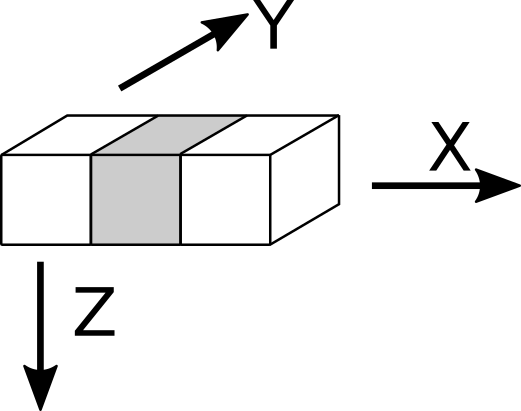
\includegraphics[width=0.7\textwidth]{drawings/buffer-ex2-no-buffer.png}
		\caption{Example 2: Stencil Operator.}
		\label{fig:buffer-ex2-no-buffer}
	\end{minipage}
	\begin{minipage}{.5\columnwidth}
		\centering
		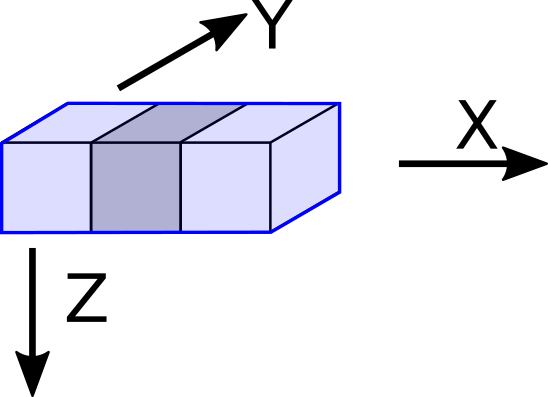
\includegraphics[width=0.7\textwidth]{drawings/buffer-ex2-buffer.png}
		\caption{Example 2: Internal Buffer laid over the Stencil.}
		\label{fig:buffer-ex2-buffer}
	\end{minipage}
\end{figure}


This number can also be derived by computing the difference between the highest and the lowest access index and adding one. 
\begin{align}
\text{max index} - \text{min index} + 1 = [i, j, k+1] - [i, j, k-1] + 1 = [0, 0, 2] + 1
\end{align}


\subparagraph{Example 3: 2D Stencil}
Our third example consists of a stencil that sums up its direct neighbors in the X-Y plane.
\begin{align}
\text{out}(i, j, k) = \text{in}(i, j, k) + \text{in}(i, j, k-1) + \text{in}(i, j, k+1) + \text{in}(i, j-1, k) + \text{in}(i, j+1, k)
\end{align}
Therefore, the stencil looks like a cross in the X-Y plane (figure \ref{fig:buffer-ex3-no-buffer}). \\
The internal buffer size of such a stencil is not a static number of elements anymore, but depends on the actual dimension sizes since the buffer is spread over a whole dimension. Using the graphic, you can verify that the buffer size of this specific stencil is 2*X + 1. 
\begin{figure}[h]
	\begin{minipage}{.5\columnwidth}
		\centering
		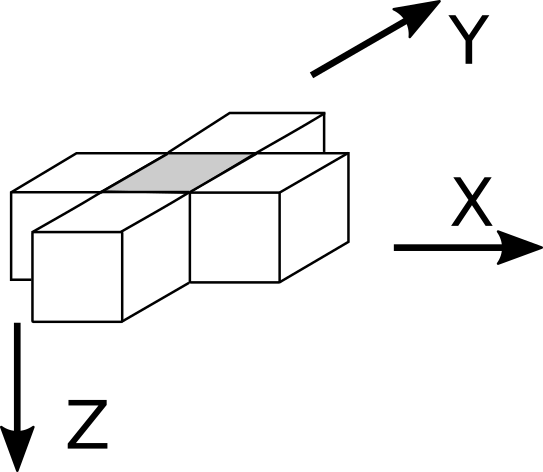
\includegraphics[width=0.7\textwidth]{drawings/buffer-ex3-no-buffer.png}
		\caption{Example 3: Stencil Operator.}
		\label{fig:buffer-ex3-no-buffer}
	\end{minipage}
	\begin{minipage}{.5\columnwidth}
		\centering
		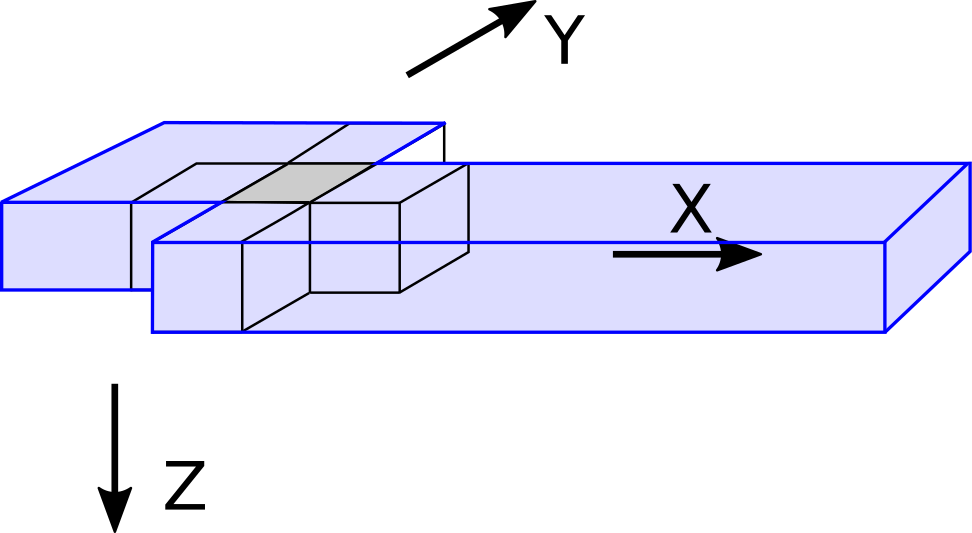
\includegraphics[width=1.0\textwidth]{drawings/buffer-ex3-buffer.png}
		\caption{Example 3: Internal Buffer laid over the Stencil.}
		\label{fig:buffer-ex3-buffer}
	\end{minipage}
\end{figure}


This number can also be derived by computing the difference between the highest and the lowest access index and adding one. 
\begin{align}
\text{max index} - \text{min index} + 1 = [i, j+1, k] - [i, j-1, k] + 1 = [0, 2, 0] + 1
\end{align}


\subparagraph{Example 4: 3D Stencil}
Our fourth example consists of a stencil that adds the center element with its neighbor in the Z dimension, which represents the outermost loop.
\begin{align}
\text{out}(i, j, k) = \text{in}(i, j, k) + \text{in}(i+1, j, k)
\end{align}
Therefore, the corresponding stencil looks like two cubes stacked above each other. \\
This time the buffer is even spread over two dimensions (i.e. layer of the X-Y plane. And has the size of X*Y + 1. 
\begin{figure}[h]
	\begin{minipage}{.5\columnwidth}
		\centering
		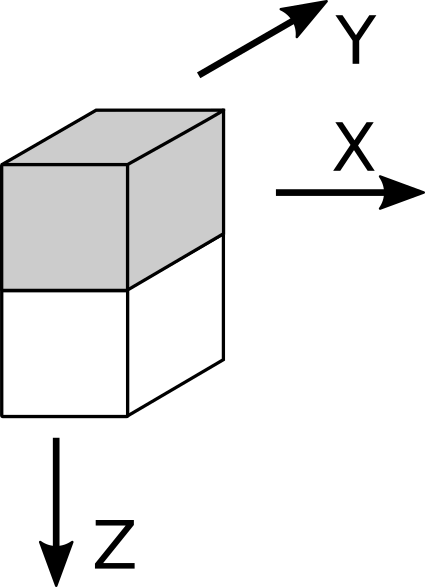
\includegraphics[width=0.5\textwidth]{drawings/buffer-ex4-no-buffer.png}
		\caption{Example 4: Stencil Operator.}
		\label{fig:buffer-ex4-no-buffer}
	\end{minipage}
	\begin{minipage}{.5\columnwidth}
		\centering
		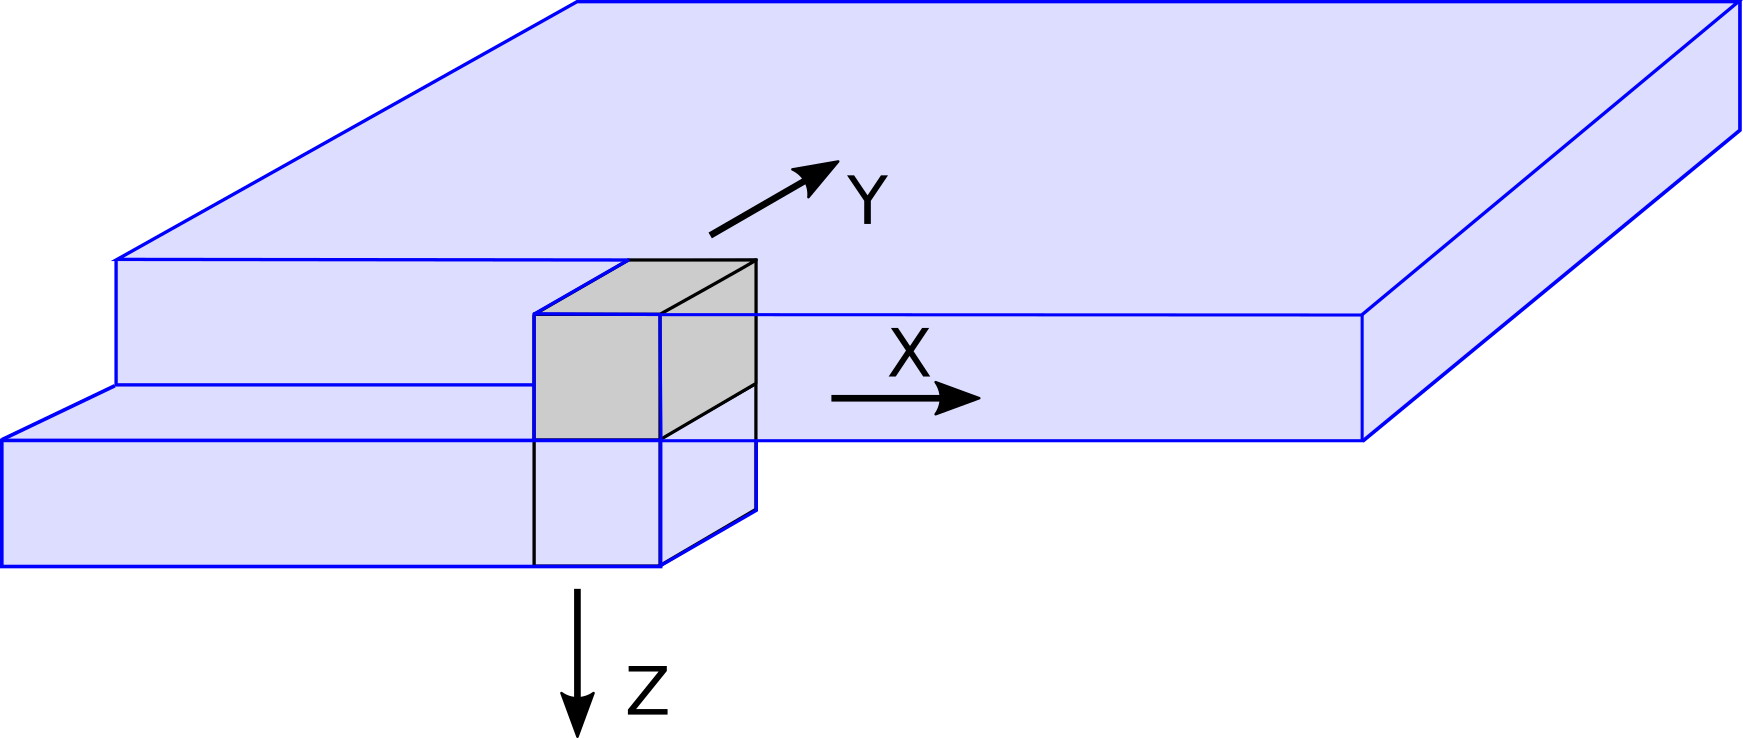
\includegraphics[width=1.0\textwidth]{drawings/buffer-ex4-buffer.png}
		\caption{Example 4: Internal Buffer laid over the Stencil.}
		\label{fig:buffer-ex4-buffer}
	\end{minipage}
\end{figure}

This number can also be derived by computing the difference between the highest and the lowest access index and adding one. 
\begin{align}
\text{max index} - \text{min index} + 1 = [i+1, j, k] - [i, j, k] + 1 = [1, 0, 0] + 1
\end{align}


\subparagraph{}
We can conclude that the internal buffer size can be computed in general using the following formula: \\
\begin{align}
\text{max index} - \text{min index} + 1
\end{align}


\subparagraph{Dimensional Notation} 
We refer to this notation of square brackets as the dimensional notation. This format is internally used in StencilFlow since it has the great benefit of being independent of the actual problem dimensions.  
The relation from the dimensional form to an absolute value is given by:
\begin{lstlisting}[showstringspaces=false, frame=single, language=Python]  
given: 
input dimensions [X,Y,Z]   
value in dimensional format: [a,b,c]
absolute size: x + X*b + X*Y*a = c + X*(b  + Y*a)
\end{lstlisting}



\subsection{Stencil Program}
The stencil program graph represents the highest level of abstraction of the stencil program. It is required to represent dependencies between different kernels and computes global properties combined from the individual stencils.


\paragraph{Stencil Program Graph}
The graph consists of input, kernel and output nodes. The input nodes represents the actual data array inputs, the kernel nodes represent stencil computations and the output nodes store the result of the computation. Edges between them are called channels and provide forwarding and buffer functionality for the pipeline. 
\begin{figure}[h]
	\centering
	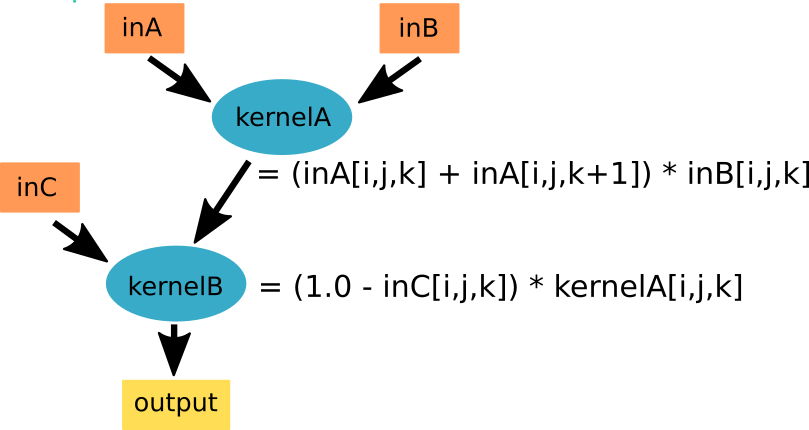
\includegraphics[height=16em]{drawings/approach-stencil-program.png}
	\caption{Example Kernel Chain Graph.}
	\label{fig:approach-stencil-program2}
\end{figure}


\paragraph{Latency}
The critical path latency of the stencil program graph is an important metric to compute the actual runtime of the program in hardware. Given the design frequency, the (theoretical) runtime is: $\frac{(critical\_path\_length + X*Y*Z)}{frequency}$. \\
The critical path computation is identical to the calculation for the compute graph. We can assign latency zero to the output nodes and walk up the tree to the inputs while adding the critical kernel latency computed by the ComputeGraph.



\paragraph{Delay Buffer}
We call the second type of buffering required to run a fully pipelined design delay buffer (beside the internal buffer described in the kernel section \ref{para:internal-buffer}). As the name suggest, its purpose is to latch intermediate data till the kernel is ready to read from the channel. This data dependency arises at the inter-kernel-level, which is why the stencil program graph has to take care of this. The following example illustrates a case where this is required.\\
The output of kernelA for kernelD is ready some time before the data stream from kernelC to kernelD arrives. Since kernelD cannot start processing the input data from kernelA, but rather has to wait for the data from kernelC, we have to introduce a delay buffer at the edge from A to D. The size of this delay buffer is (assuming field accesses of D from C and A are identical e.g kernelD[i,j,k] = kernelA[i,j,k] + kernelC[i,j,k]) given by the latency of the path kernelA-kernelB-kernelC-kernelD.   
\begin{figure}[h]
	\begin{minipage}{.5\columnwidth}
		\centering
		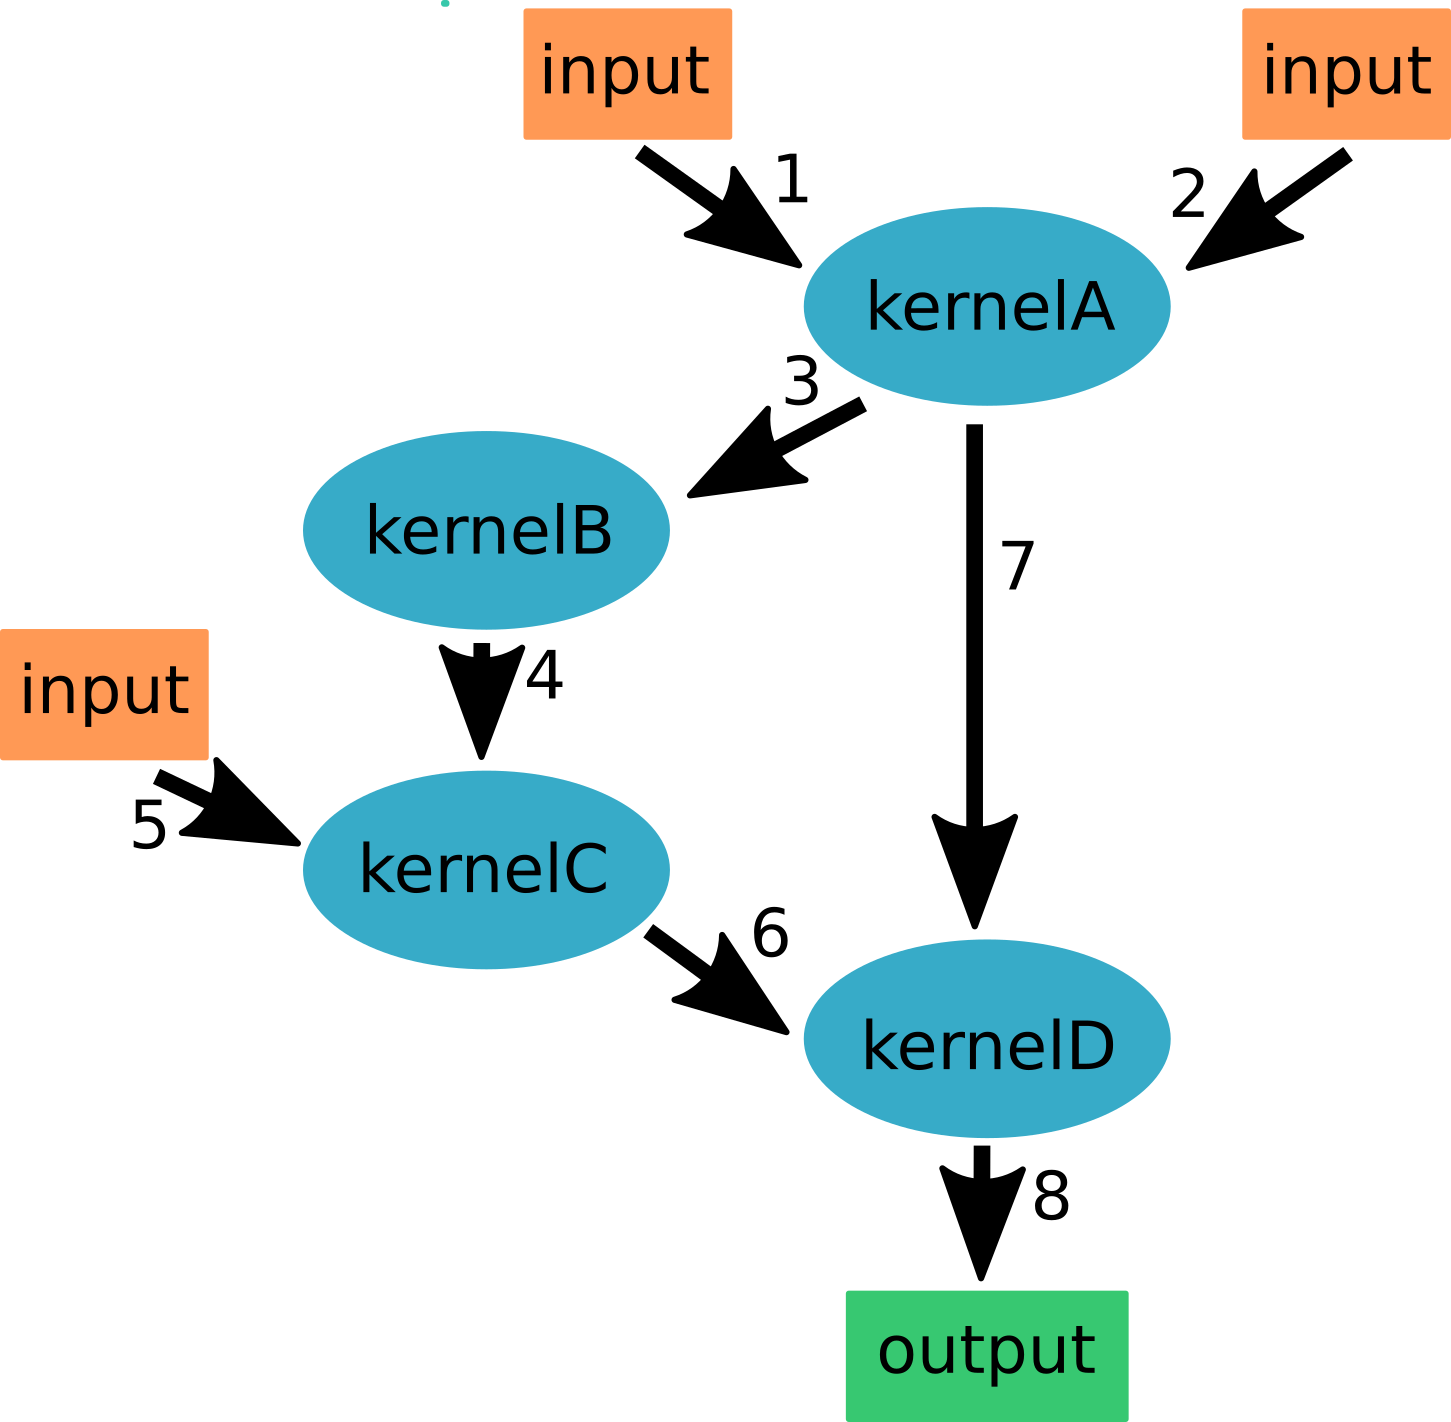
\includegraphics[height=16em]{drawings/model-delay-buffer1.png}
		\caption{Example stencil program.}
		\label{fig:model-delay-buffer}
		\vspace{1em}
	\end{minipage}
	\begin{minipage}{.5\columnwidth}
		\centering
		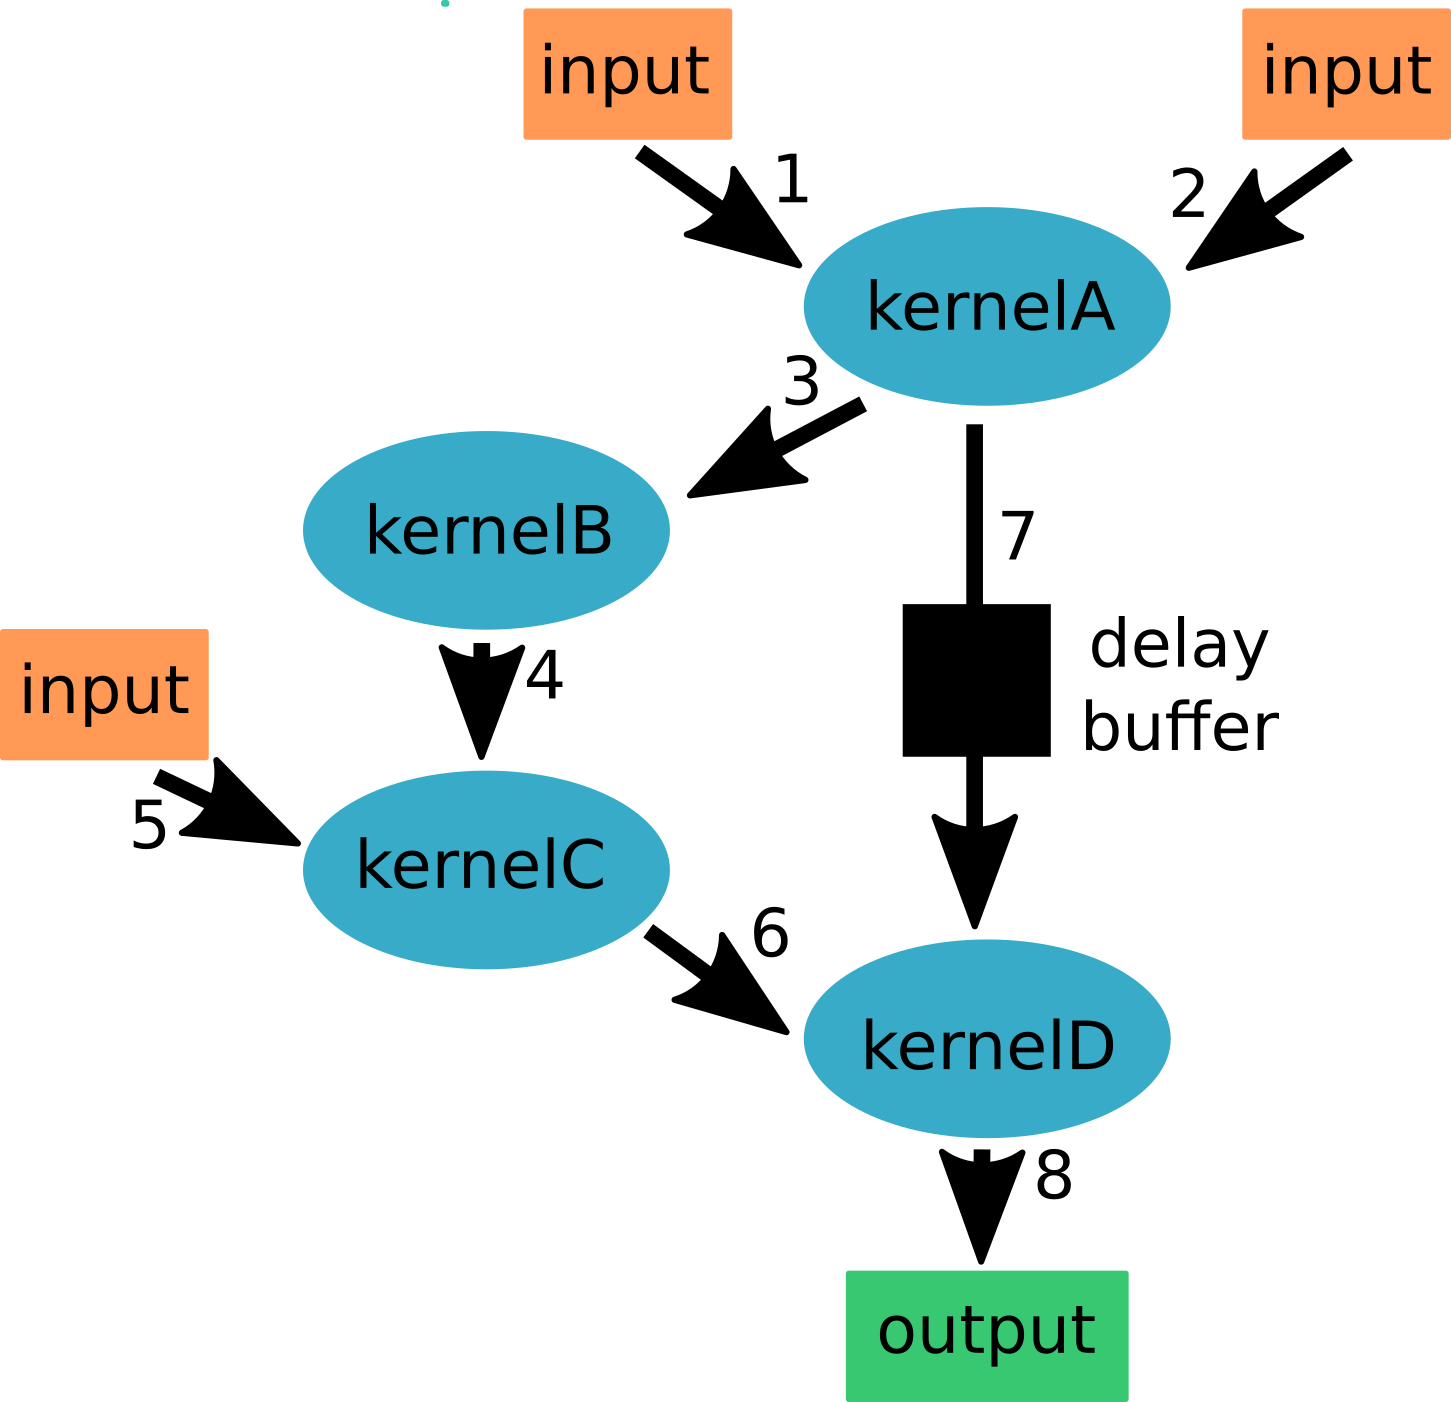
\includegraphics[height=16em]{drawings/model-delay-buffer2.png}
		\caption{Example stencil program with delay buffer.}
		\label{fig:model-delay-buffer2}
	\end{minipage}
\end{figure}



\section{FPGA Model}
Since we are dealing with a memory bound problem and seek to optimize for maximal throughput, our model is very data-centric, especially since todays state-of-the-art FPGAs offer such a huge amount of hardened digital signal processors (DSPs) (e.g. 10 TFLOP/s peak 32-bit floating point operations on a Stratix 10 \label{label25}). Therefore we assume that we are limited by either on-chip memory capacity or off-chip memory bandwidth.
\begin{figure}[h]
	\centering
	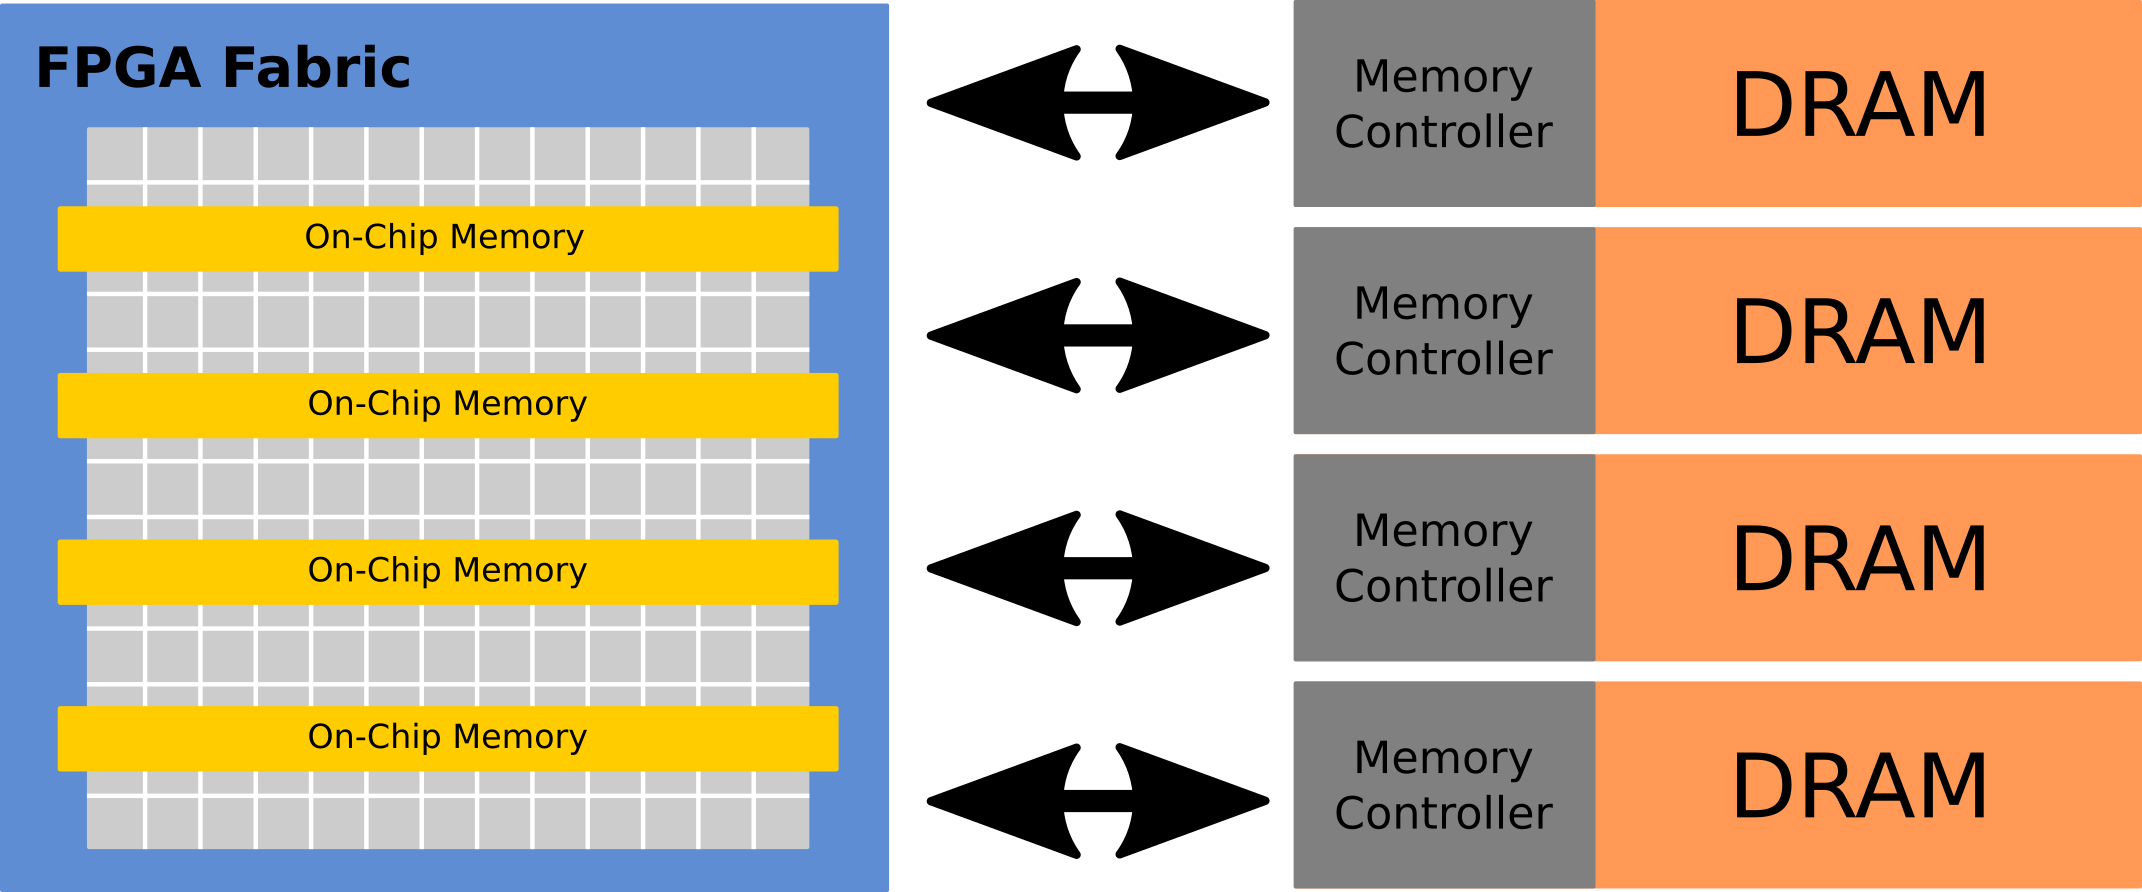
\includegraphics[height=12em]{drawings/optimizer-memory-system.png}
	\caption{Basic memory model: Fast on-chip memory, slow DRAM memory and memory bandwidth.}
	\label{fig:optimizer-memory-system}
\end{figure}


\subsection{Fast and Slow Memory}
Since we fully pipeline the whole stencil program, we need to lay out all the internal and delay buffers in memory. While the fast on-chip memory of the FPGA has very low latency/high throughput and a low energy footprint compared to the slow DRAM memory (including the data path to the DRAM), it is a limited resource and we have to carefully choose which buffers we allocate in fast memory and which we better swap out to the slow memory.


\subsection{Memory Bandwidth}
Furthermore, even before having filled up the whole DRAM with buffers, we might run into the issue that we run out of bandwidth between the DRAM and the FPGA fabric. Therefore, memory bandwidth is a key metric too, which we have to take into account in the optimization process.




\section{Hardware Mapping: DaCe}
Despite our high-level optimization, it has been shown that FPGA designs can gain significant performance increase \cite{label57} if the HLS design has been further optimized and equipped with the suitable pragmas and formulations. \\
Therefore, we decided to decouple the high-level representation from the lower-level and use DaCe \footnote{https://github.com/spcl/dace}, which is able to compile FPGA code with high utilization and performance from the intermediate representation, the so called Stateful DataFlow multiGraph (SDFG) \cite{label57}. \\
The SDFG intermediate representation is a directed graph of directed acyclic multi graphs, where the nodes represent computations and storage while the edges represent data movement. Figure \ref{fig:dace-sdft-syntax} summaries all graph primitives of the stateful dataflow multigraph. \\ 
\begin{figure}[h]
	\centering
	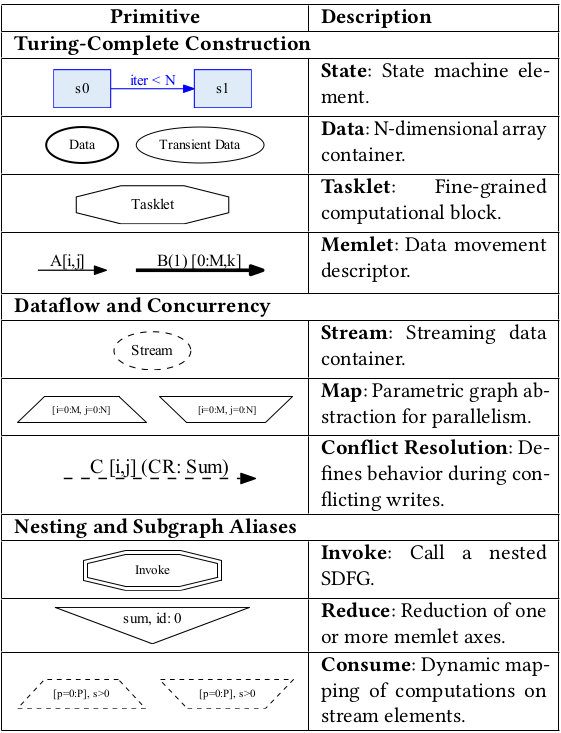
\includegraphics[height=16em]{images/dace-sdft-syntax.png}
	\caption{SDFG primitives syntax and description. \cite{label57}}
	\label{fig:dace-sdft-syntax}
\end{figure}

In order to get a better understanding we look at the transformation of vector addition from python code to the SDFG graph representation. 
\begin{minted}{python}
def vector_add(A, B):
  return list(map(lambda x,y: x+y, A, B))
\end{minted}
The corresponding graph starts with the two N-dimensional array containers A and B, which are connected by a data movement descriptor (memlet) through a map with the fine-grained computational block (tasklet). The map primitive splits the N-dimensional problem into N parallel 1-dimensional sub-problems in order to exploit the implicit parallelism. This is illustrated in figure \ref{fig:dace-vetor-add-n3} for the case N=3. The tasklet describes this element-wise computation:
\begin{align}
\text{C}[i] = \text{A}[i] + \text{B}[i]
\end{align}
The resulting is then mapped back to the N-dimensional form and finally stored in the output data container C as shown in figure \ref{fig:dace-vector-add}.
\begin{figure}[H]
	\begin{minipage}{.5\columnwidth}
		\centering
		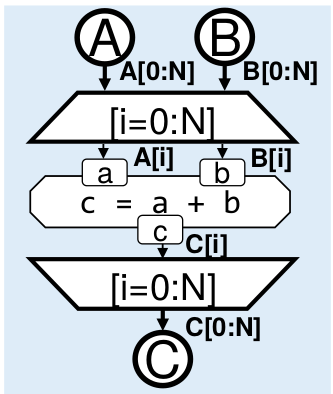
\includegraphics[height=12em]{images/dace-vector-add.png}
		\caption{SDFG in parametric form. \cite{label57}}
		\label{fig:dace-vector-add}
		\vspace{1.5em}
	\end{minipage}
	\begin{minipage}{.5\columnwidth}
		\centering
		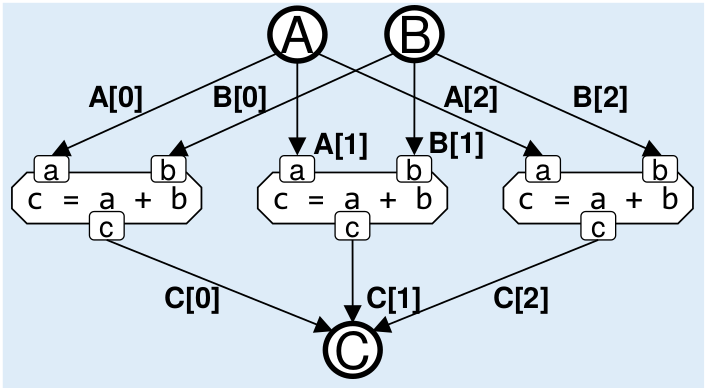
\includegraphics[height=12em]{images/dace-vetor-add-n3.png}
		\caption{SDFG expanded for N=3. \cite{label57}}
		\label{fig:dace-vetor-add-n3}
	\end{minipage}
\end{figure}

This general graph representation builds the foundation for the transformation and optimization to different hardware platforms, which makes DaCe a very powerful toolbox. It incorporates many optimization techniques such as tiling and fusion in order to generate efficient code for the specific platform. Figure \ref{fig:dace} shows the complete transformation process form the domain specific high-level program to the hardware-specific optimized design.
\begin{figure}[h]
	\centering
	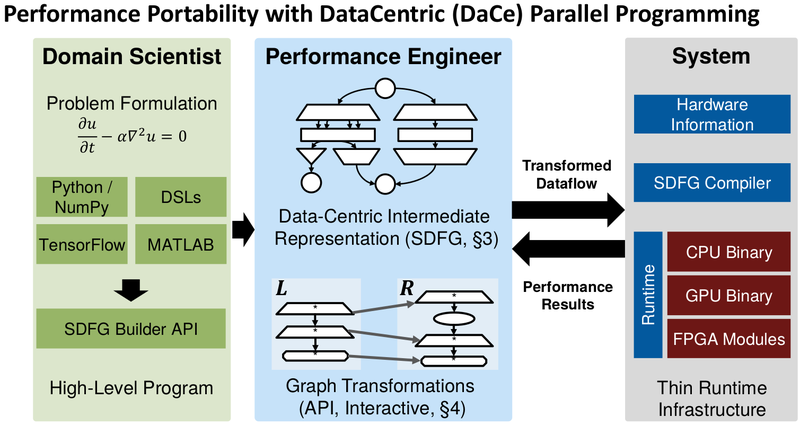
\includegraphics[width=1.0\textwidth]{images/dace.png}
	\caption{ \textit{Presentation Slide: Data-Centric Parallel Programming,Torsten Hoefler, invited talk at ISC’19, Frankfurt, Germany}}
	\label{fig:dace}
\end{figure}




\section{Conclusion}
So far, we have seen that the actual problem to solve is trading the different compromise in resource allocation against each other to find a feasible and well performing design. The foundation for such an optimization has been laid down in this chapter by formalizing the analysis of resource requirements. In the next chapter, we will have a look on how we can formalize a objective and find the (theoretical) optimal solution within our specific assumptions.












